\section{问题三　固定参考标记的角度标定精度}
\subsection{圆周角误差的达标概率}
仪器观测一个位置已知、距离为 \(R=40\) 米的固定参考标记。累计移动距离达到 \(s\) 米后，两个坐标方向的误差相互独立，均服从 \(N(0,\sigma^2)\)，其中 \(\sigma=0.30+0.02s\)。仪器零偏误差和控制误差也相互独立，标准差分别为 \(0.8^\circ\) 和 \(0.6^\circ\)，合成标准差为 \(\tau=1^\circ\)。取三个相互独立的标准正态变量 \(X,Y,Z\)，总角误差可以写成
\begin{equation}
 D=\operatorname{wrap}_{[-\pi,\pi)}\!\left[
 \operatorname{atan2}(\sigma Y,R+\sigma X)+\tau Z\right].
\end{equation}
两个坐标误差的分布均关于零对称，因此交换其中任一误差分量的正负号约定不影响角误差的分布。令容差 \(\delta=5^\circ\)，要求达标概率 \(p(\sigma)=\Pr(|D|\leq\delta)\geq0.95\)。

给定 \(Z=z\)，将带坐标误差的参考向量旋转 \(g=\tau z\)，再除以 \(\sigma>0\)。由于坐标误差在平面内各向同性，该向量的协方差矩阵为单位阵，均值为 \((m,n)=(R/\sigma)(\cos g,\sin g)\)。设标准化后水平方向的残差为 \(u\)。对给定的 \(u\)，达标要求横坐标 \(m+u\) 为正，且纵坐标落在 \([-h,h]\) 内，其中 \(h=(m+u)\tan\delta\)。记标准正态分布的密度函数和分布函数为 \(\phi\) 和 \(\Phi\)，则
\begin{equation}
 p(\sigma)=\int_{\mathbb R}\!\phi(z)
 \int_{-m}^{\infty}\!\phi(u)
 \{\Phi(h-n)-\Phi(-h-n)\}\,du\,dz .
 \label{eq:sector}
\end{equation}
上述达标事件对应平面中的一个扇形，因此角度跨过 \(\pm\pi\) 的折返点时，判据仍然成立。

为证明临界值唯一，对不同 \(\sigma\) 使用同一组 \(X,Y\)。坐标误差引起的角偏差的绝对值为 \(\operatorname{atan2}(|Y|,R/\sigma+X)\)，几乎必然随 \(\sigma\) 严格增大。独立仪器误差服从以零为中心的卷绕正态分布。由文献~\cite{theta} 的 theta 函数乘积公式可知，其密度随到零点的圆周距离增大而严格递减。对于具有这一性质的偶密度 \(f\)，将半宽为 \(\delta\) 的弧段中心从零移至圆周距离 \(a\) 处时，弧内概率对 \(a\) 的导数为 \(f(a+\delta)-f(a-\delta)\leq0\)，两端点均按圆周角取值。由此可得 \(p(\sigma)\) 严格递减，方程 \(p(\sigma)=0.95\) 的根就是允许的最大坐标误差标准差。

\clearpage
\subsection{距离上限、独立模拟与方差贡献}
对式~\eqref{eq:sector} 采用 96 点高斯--勒让德求积，再求解 \(p=0.95\)，得到
\begin{equation}
 \sigma_* = 1.636745169\,\mathrm m,\qquad
 s_*=(\sigma_*-0.30)/0.02=66.83725843\,\mathrm m .
\end{equation}
若要求累计移动 80 米时依然达标，对误差模型 \(\sigma(s)=a+bs\)，其中 \(a,b\geq0\)，充要条件为 \(a+80b\leq\sigma_*\)。例如，保持 \(a=0.30\,\mathrm m\) 时，须有 \(b\leq(\sigma_*-0.30)/80\simeq0.016709315\)。标称参数给出 \(\sigma(80)=1.90\,\mathrm m\)，此时达标概率为 \(91.5068\%\)。

\begin{table}[H]\centering
\caption{积分结果与直接模拟结果。每个距离分别采用 200 万次独立试验。}\label{tab:noise}
\NoiseTable
\end{table}
\begin{figure}[H]\centering
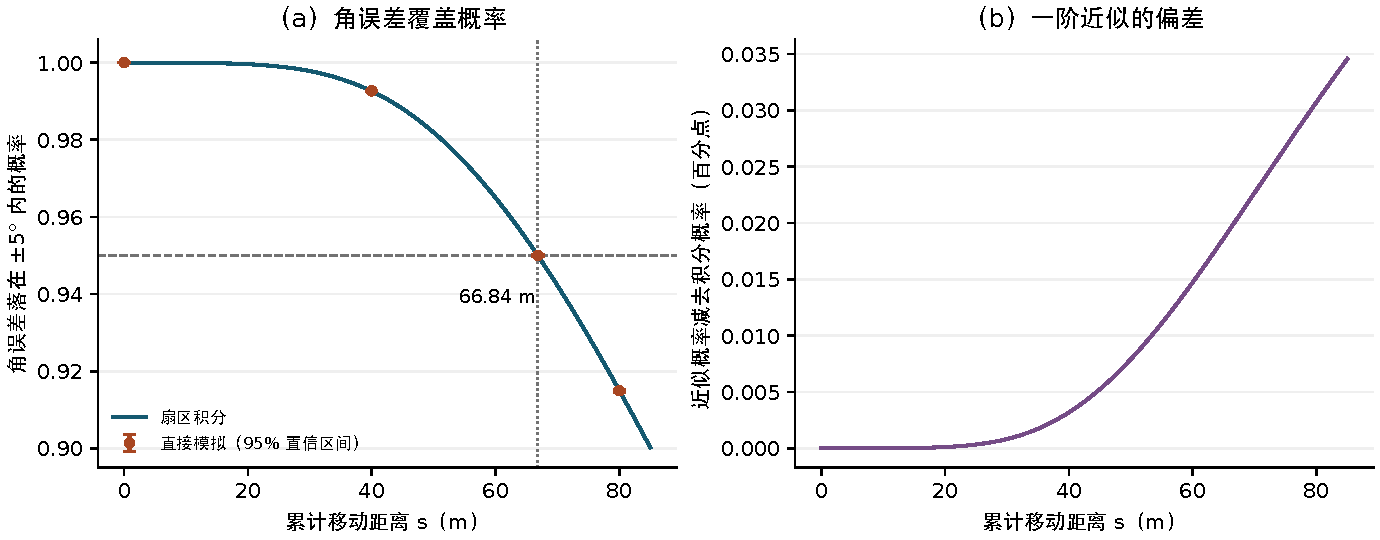
\includegraphics[width=.93\linewidth,height=.25\textheight,keepaspectratio]{q3_validation.pdf}
\caption{达标概率随累计移动距离的变化。右图单列一阶近似与积分结果之差。}\label{fig:noise}
\end{figure}
模拟分别对两个坐标误差分量以及零偏、控制两项仪器误差抽样。先用 \(\operatorname{atan2}\) 计算坐标偏差产生的角度，再加上仪器误差，将结果折回规定区间。表~\ref{tab:noise} 中的区间是各距离下分别计算的 95\% Wilson 置信区间~\cite{wilson}。不同距离共用同一组随机数，以减小距离间比较的抽样波动。将每个正态积分都截断在正负十个标准差内，舍去的概率不超过 \(4\Phi(-10)<3.1\times10^{-23}\)。改用 64 点或 128 点求积，所得 \(\sigma_*\) 与 96 点结果的差均小于 \(2\times10^{-13}\,\mathrm m\)。

在标称参考方向处作一阶线性化，角误差方差为 \(V_D\approx(\sigma/R)^2+\tau^2\)，单位为弧度平方。该近似给出的累计移动距离上限为 66.92230 米，比积分所得上限高 0.08504 米。在精确临界点处，按一阶模型分解总方差，坐标误差、零偏误差、控制误差分别占 84.61\%、9.85\% 和 5.54\%。若仅考察仪器误差，零偏和控制误差分别占其方差的 64\% 和 36\%。因此，在本算例的临界点附近，优先减小坐标漂移对降低总方差的一阶作用最大。

\clearpage
\section{问题四　扰动下的检修工单重排}
\subsection{第 8 分钟可以调整哪些工单}
两种策略都从队列 B--C--D--A--E 开始。第 8 分钟到达的通知给出新增工单及其工时，并在复核台停机时说明恢复时刻。此后不再发生其他扰动。此时 B 和 C 的检测都已开始，它们在队列中的位置固定。若停机打断了正在进行的复核，恢复后优先完成该单的剩余工作。恰好在第 36 分钟完成的工单计入按期完成数。

保留原序时，把新增工单依次追加到队尾。允许重排时，枚举尚未开始检测的工单的全部排列，原序也在其中。若改变顺序，需要在检测工位下一次空闲时占用它两分钟更新队列，在本例中为第 12 至 14 分钟。更新期间复核台可以继续工作。保留原序无需更新队列。

对每个可行顺序，程序按两道工序的递推关系计算时间线。若某单的复核跨过停机区间，则分别记录停机前后的两个工作时段。令 \(k=\#\{j:C_j\leq36\}\)，\(N\) 为截至通知时已公布的工单总数，含新增工单。先选取按期完成比例 \(k/N\) 较高的方案，比例相同再选实际清空时刻 \(C_{\max}\) 较早的方案。两项均相同时优先保留原序，此后按各单完工时刻之和最小、工单编号字典序择定代表解。另外记录以窗口终点封顶的末次完工时刻，只要有工单逾期，该指标即记为 36 分钟。实际清空时刻仍能区分封顶指标相同的逾期方案。
\begin{table}[H]\centering
\caption{相同扰动下的两种策略。按期完成数衡量截止前的交付量，实际清空时刻衡量全部工作结束的时间。}\label{tab:events}
\ScenarioTable
\end{table}
S0 为无扰动对照。S1 新增 F，S2 的复核台停机 8 分钟，S3 同时发生这两项扰动。S4 同时新增 F 和 G，S5 在此基础上再加 12 分钟停机。六个场景分别考察新增工作、产能暂时下降及二者的共同作用，不对各场景的发生概率作假设。

\clearpage
\subsection{重排在哪些场景下有收益}
\begin{figure}[H]\centering
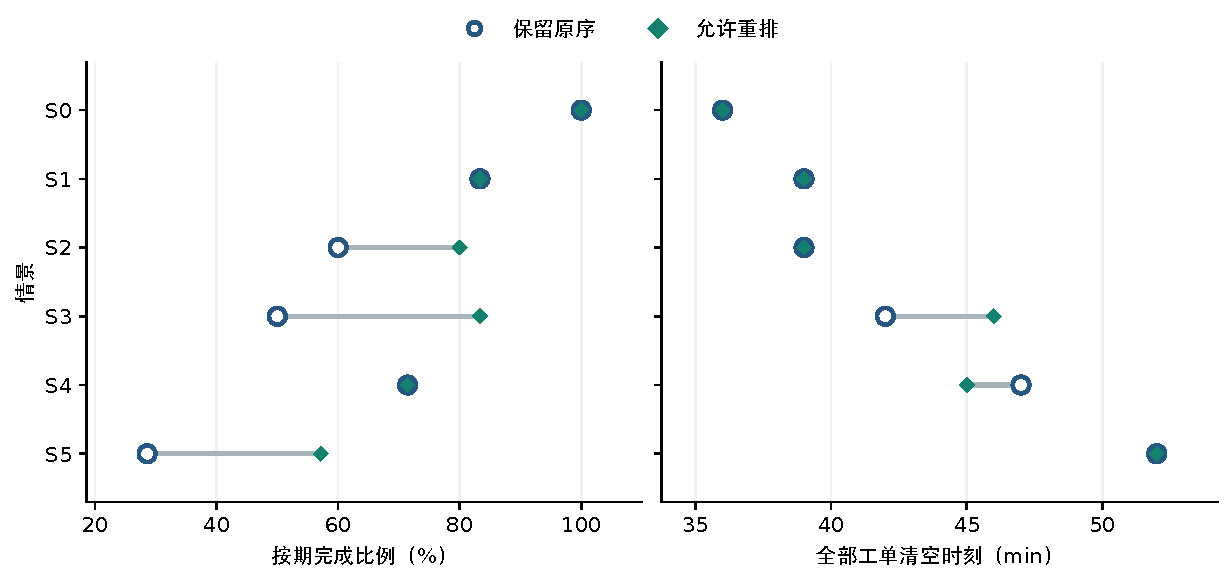
\includegraphics[width=.94\linewidth,height=.32\textheight,keepaspectratio]{schedule_comparison.pdf}
\caption{六个场景的策略比较。按期完成比例越高越好，实际清空时刻越早越好。}\label{fig:schedule}
\end{figure}
在 S0 和 S1 中，最优策略都保留原序。在 S2 中，将 E 提前可使按期完成数从 3 单增至 4 单，实际清空时刻不变。在 S3 中，将短工单 E 和 F 提前后，按期完成数从保留原序时的 3 单增至 5 单，实际清空时刻也从第 42 分钟推迟到第 46 分钟。若管理者更看重最后一单的完成时间，这一取舍就可能改变。

S4 体现了第二项评分指标的作用。两种策略都能按期完成 7 单中的 5 单，重排使清空时刻从第 47 分钟提前到第 45 分钟。在 S5 中，重排能按期完成 7 单中的 4 单，保留原序只能按期完成 2 单，两者均在第 52 分钟清空。允许重排的候选集包含按实际成本执行的原序，因此在本题规定的两级排序下，允许重排所得最优分数至少与保留原序相同。

\noindent\textbf{队列更新时间的敏感性。}\SensitivityText

\noindent\textbf{计算核验。}六个场景分别枚举 6、24、6、24、120、120 个候选后缀。对每个候选顺序，另以一分钟为步长回放过程，逐项核对剩余工时、工位占用和事件递推给出的各个区间。附录列出每个场景中两种策略的完整时间线。以上比较均以通知给出的恢复时刻准确为前提。

\clearpage
\subsection{在维修时长未知时决定队列}
现在设第 8 分钟时，车间知道新增了哪些工单，也知道复核台已停机，但必须在获知实际维修时长 \(L\) 前一次性选定剩余队列。已固定的前缀 B--C、两分钟队列更新时间、第 36 分钟截止和各工单工时保持不变。为考察提前获知维修时长的价值，令 4 至 16 分钟的 13 个整数时长等概率出现。该分布用于设定压力试验，未经现场故障数据拟合。

当 \(L=\ell\) 时，用 \(k(\pi,\ell)\) 表示队列 \(\pi\) 的按期完成数，\(C(\pi,\ell)\) 表示实际清空时刻。给定新增工单集合后，应对每个可能的时长采用同一个 \(\pi\)。若各时长的概率权重为 \(w_\ell\)，目标为
\[
 \mathop{\mathrm{lex\,min}}_{\pi}\left(
  -\sum_{\ell=4}^{16} w_\ell k(\pi,\ell),\
   \sum_{\ell=4}^{16} w_\ell C(\pi,\ell)\right).
\]
先最大化期望按期完成数，再从达到该最大值的队列中选取期望清空时刻最早的一组。比较的规则包括保留原序、将剩余工单按两道工序总工时从短到长排序、将平均维修时长代入模型求解，以及按上述双重期望目标求解。另设完全信息基准，允许对每个实际维修时长分别选取最优队列。各方法只要改变原序，均承担相同的队列更新开销。

\begin{table}[H]\centering
\caption{新增一张工单 F 时的策略比较。期望值按 13 个等概率维修时长计算。}
\RecoveryTable
\end{table}
新增 F 时，利用完整时长分布优化和代入平均维修时长得到相同的队列。若能提前知道实际维修时长，期望按期完成数仍然相同，但平均清空时刻可比预先选定队列提前 1.15 分钟。若只有复核台停机，没有新增工单，完整分布优化的期望按期完成数为 \(49/13=3.769\) 单，代入平均时长的结果为 \(48/13=3.692\) 单。即使已知各项工时的均值，直接代入均值仍可能错过最优队列。

\clearpage
\subsection{在哪些维修时长下值得重排}
\begin{figure}[H]\centering
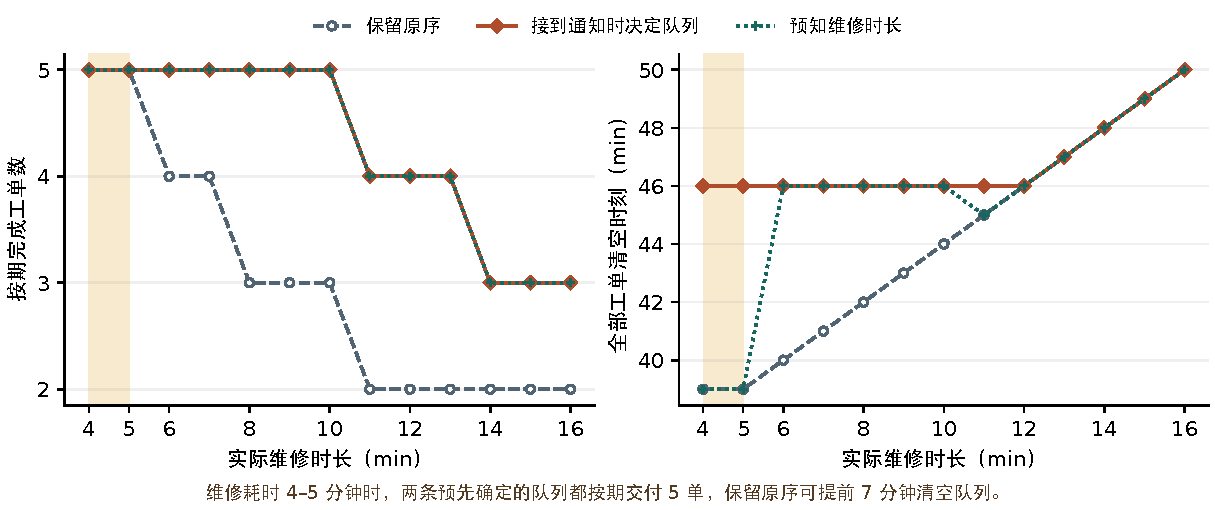
\includegraphics[width=.94\linewidth,height=.30\textheight,keepaspectratio]{uncertain_recovery.pdf}
\caption{新增工单 F。两条固定队列在通知时选定；完全信息基准可以预知维修时长。}\label{fig:repair}
\end{figure}
图~\ref{fig:repair} 中，若采用 B--C--E--F--A--D，维修耗时 8 至 13 分钟，重排恰好比保留原序多按期交付 2 单。这涵盖 13 个时长中的 6 个。如果维修仅用 4 或 5 分钟，两种队列都能按期完成 5 单，但原序在第 39 分钟清空，重排要到第 46 分钟。在其余 5 个时长下，重排比原序多按期交付 1 单。综合各时长，重排平均多按期交付 \(17/13=1.31\) 单，实际清空时刻平均推迟 \(35/13=2.69\) 分钟。

设每多按期交付一单，车间愿意让最后一单晚 \(v\ge0\) 分钟完成。在全部 24 条可行队列中最小化 \(\mathbb E[C]-v\mathbb E[k]\)。每条队列的成本都是 \(v\) 的一次函数。将 13 种维修时长的清空时刻与按期单数分别求和，可得到 13 倍成本的整数系数，由此得到表~\ref{tab:value} 的精确分界。
\begin{table}[H]\centering
\caption{新增 F、各维修时长等概率时的最低成本队列。在两个分界点，相邻两条队列并列最优。}\label{tab:value}
\small\begin{tabular}{@{}lcrr@{}}\toprule
可接受延迟 \(v\)（分钟/单）& 队列 & 期望按期单数 & 平均清空时刻（分钟）\\\midrule
\TradeoffRows
\bottomrule\end{tabular}
\end{table}
从原序 BCDAEF 改为 BCEFDA，平均多交付 \(12/13\) 单，只需多等 \(5/13\) 分钟，折合每单 \(5/12\) 分钟。再改为 BCEFAD，平均多交付 \(5/13\) 单，还需多等 \(30/13\) 分钟，折合每单 6 分钟。若只比较首尾两条队列，交点为 \(35/17\approx2.06\) 分钟/单；在这一位置，中间队列 BCEFDA 的成本严格更低。

对按期单数优先的目标，再按 \(17-\ell\) 和 \(\ell-3\) 为各维修时长赋予相对权重。平均维修时长分别为 8 和 12 分钟时，新增 F 的最优固定队列仍为 BCEFAD，期望按期单数分别为 4.70 和 3.91。三个到单情景共 \(13(6+24+120)=1950\) 个队列与时长组合，均经逐分钟回放核对。
